Para esta situación podriamos realizar el mismo desglose de variantes para llegar a varias posibles soluciones con diferentes complejidades. Pero para este caso ya podemos ser más directos. 

Suponga que las filas y columnas de la cuadrícula están numeradas del $0$ al $n$, y que el $value[y][x]$ es igual al valor del cuadrado($y$,$x$). Sea sum($y$,$x$) la suma máxima en un camino desde la esquina superior izquierda hasta el cuadrado ($y$, $x$). Entonces, sum($n-1$, $n-1$) nos dice la suma máxima desde la esquina superior izquierda hasta la esquina inferior derecha. Por ejemplo, en la cuadrícula en la sección introductoria, suma(5,5) = 67. Ahora podemos usar la fórmula:

$$sum(y,x) = max(sum(y,x-1),sum(y-1,x))+value[y][x]$$

Que se basa en la observación de que un camino que termina en el cuadrado($y$,$x$) puede provenir del cuadrado($y$,$x-1$) o del cuadrado ($y-1$,$x$) vea figura de abajo:

% TODO: \usepackage{graphicx} required
\begin{figure}[h!]
	\centering
	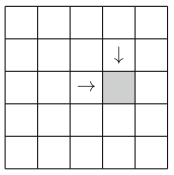
\includegraphics[width=0.3\linewidth]{img/grid_path_ii}
	\label{fig:gridpathii}
\end{figure} 

Así, seleccionamos la dirección que maximiza la suma. Suponemos que suma($y$, $x$) = $0$ si $y < 0 $ o $x < 0$, por lo que la fórmula recursiva también funciona para los cuadrados situados más a la izquierda y más arriba. Ya visto que la fórmula es la correcta la misma puede ser implementada aplicando los mismos enfoques que fueron utilizados para resolver la cantidad de caminos. 

